% This is "sig-alternate.tex" V2.1 April 2013
% This file should be compiled with V2.5 of "sig-alternate.cls" May 2012
%
% This example file demonstrates the use of the 'sig-alternate.cls'
% V2.5 LaTeX2e document class file. It is for those submitting
% articles to ACM Conference Proceedings WHO DO NOT WISH TO
% STRICTLY ADHERE TO THE SIGS (PUBS-BOARD-ENDORSED) STYLE.
% The 'sig-alternate.cls' file will produce a similar-looking,
% albeit, 'tighter' paper resulting in, invariably, fewer pages.
%
% ----------------------------------------------------------------------------------------------------------------
% This .tex file (and associated .cls V2.5) produces:
%       1) The Permission Statement
%       2) The Conference (location) Info information
%       3) The Copyright Line with ACM data
%       4) NO page numbers
%
% as against the acm_proc_article-sp.cls file which
% DOES NOT produce 1) thru' 3) above.
%
% Using 'sig-alternate.cls' you have control, however, from within
% the source .tex file, over both the CopyrightYear
% (defaulted to 200X) and the ACM Copyright Data
% (defaulted to X-XXXXX-XX-X/XX/XX).
% e.g.
% \CopyrightYear{2007} will cause 2007 to appear in the copyright line.
% \crdata{0-12345-67-8/90/12} will cause 0-12345-67-8/90/12 to appear in the copyright line.
%
% ---------------------------------------------------------------------------------------------------------------
% This .tex source is an example which *does* use
% the .bib file (from which the .bbl file % is produced).
% REMEMBER HOWEVER: After having produced the .bbl file,
% and prior to final submission, you *NEED* to 'insert'
% your .bbl file into your source .tex file so as to provide
% ONE 'self-contained' source file.
%
% ================= IF YOU HAVE QUESTIONS =======================
% Questions regarding the SIGS styles, SIGS policies and
% procedures, Conferences etc. should be sent to
% Adrienne Griscti (griscti@acm.org)
%
% Technical questions _only_ to
% Gerald Murray (murray@hq.acm.org)
% ===============================================================
%
% For tracking purposes - this is V2.0 - May 2012

\documentclass{sig-alternate-05-2015}

\usepackage{amsmath}
\usepackage{algorithm}
\usepackage[noend]{algpseudocode}
\usepackage[flushleft]{threeparttable}
\usepackage{subfigure}

\newtheorem{theorem}{Theorem}

%\makeatletter
%\def\@copyrightspace{\relax}
%\makeatother

\begin{document}

%% Copyright
%\setcopyright{acmcopyright}
%%\setcopyright{acmlicensed}
%%\setcopyright{rightsretained}
%%\setcopyright{usgov}
%%\setcopyright{usgovmixed}
%%\setcopyright{cagov}
%%\setcopyright{cagovmixed}
%
%
%% DOI
\doi{}
%\doi{10.475/123_4}
%
%% ISBN
\isbn{}
%\isbn{123-4567-24-567/08/06}
%
%%Conference
%\conferenceinfo{PLDI '13}{June 16--19, 2013, Seattle, WA, USA}
%
%\acmPrice{\$15.00}
%
%%
%% --- Author Metadata here ---
%%\conferenceinfo{WOODSTOCK}{'97 El Paso, Texas USA}
%%\CopyrightYear{2007} % Allows default copyright year (20XX) to be over-ridden - IF NEED BE.
%%\crdata{0-12345-67-8/90/01}  % Allows default copyright data (0-89791-88-6/97/05) to be over-ridden - IF NEED BE.
%% --- End of Author Metadata ---

\title{Decentralized Search for Shortest Path Approximation \\
in Large-scale Complex Networks}
%\subtitle{[Extended Abstract]
%\titlenote{A full version of this paper is available as
%\textit{Author's Guide to Preparing ACM SIG Proceedings Using
%\LaTeX$2_\epsilon$\ and BibTeX} at
%\texttt{www.acm.org/eaddress.htm}}}
%
% You need the command \numberofauthors to handle the 'placement
% and alignment' of the authors beneath the title.
%
% For aesthetic reasons, we recommend 'three authors at a time'
% i.e. three 'name/affiliation blocks' be placed beneath the title.
%
% NOTE: You are NOT restricted in how many 'rows' of
% "name/affiliations" may appear. We just ask that you restrict
% the number of 'columns' to three.
%
% Because of the available 'opening page real-estate'
% we ask you to refrain from putting more than six authors
% (two rows with three columns) beneath the article title.
% More than six makes the first-page appear very cluttered indeed.
%
% Use the \alignauthor commands to handle the names
% and affiliations for an 'aesthetic maximum' of six authors.
% Add names, affiliations, addresses for
% the seventh etc. author(s) as the argument for the
% \additionalauthors command.
% These 'additional authors' will be output/set for you
% without further effort on your part as the last section in
% the body of your article BEFORE References or any Appendices.

%\numberofauthors{3} %  in this sample file, there are a *total*
%% of EIGHT authors. SIX appear on the 'first-page' (for formatting
%% reasons) and the remaining two appear in the \additionalauthors section.
%%
%\author{
%% You can go ahead and credit any number of authors here,
%% e.g. one 'row of three' or two rows (consisting of one row of three
%% and a second row of one, two or three).
%%
%% The command \alignauthor (no curly braces needed) should
%% precede each author name, affiliation/snail-mail address and
%% e-mail address. Additionally, tag each line of
%% affiliation/address with \affaddr, and tag the
%% e-mail address with \email.
%%
%% 1st. author
%\alignauthor Zheng Lu\\
       %\affaddr{Electrical Engineering and Computer Science}\\
       %\affaddr{University of Tennessee, Knoxville}\\
       %\email{zlu12@vols.utk.edu}
%% 2nd. author
%\alignauthor Yunhe Feng\\
       %\affaddr{Electrical Engineering and Computer Science}\\
       %\affaddr{University of Tennessee, Knoxville}\\
       %\email{yfeng14@vols.utk.edu}
%% 3rd. author
%\alignauthor Qing Cao\\
       %\affaddr{Electrical Engineering and Computer Science}\\
       %\affaddr{University of Tennessee, Knoxville}\\
       %\email{cao@utk.edu}
%}

\date{30 April 2016}


\maketitle
\begin{abstract}
Finding approximated shortest paths for extremely large-scale complex networks is a challenging problem, where existing works require large overhead to achieve high accuracy and diversity for estimated paths, especially for large graphs with millions of vertices. In this paper, we propose an online search approach based on preprocessed indexes, to approximate point-to-point shortest paths. The approach is able to find more accurate and diverse paths with limited index overhead and requires low search overhead. The level of accuracy and required resource can be balanced by dynamically controlling the search space to meet various application needs. Furthermore, a new heuristic index construction algorithm is introduced that can greatly increase the approximation accuracy and involve no additional index overhead. To handle extreme size graphs, we build a query processing system with our algorithm on distributed graph processing platforms. The system also supports parallel processing of online searches to achieve high throughput for a large number of queries. We evaluate our algorithm on various real-world graphs from different disciplines with up to billions of edges, and we demonstrate that our system can process hundreds of thousand queries per second on these graphs with reduced overhead.
\end{abstract}


%
% The code below should be generated by the tool at
% http://dl.acm.org/ccs.cfm
% Please copy and paste the code instead of the example below.
%
\begin{CCSXML}

<ccs2012>


<concept>

<concept_id>10002951.10002952.10002971</concept_id>
 <concept_desc>Information systems~Data structures</concept_desc>

<concept_significance>500</concept_significance>
</concept>

<concept>

<concept_id>10002951.10003227.10003351</concept_id>
 <concept_desc>Information systems~Data mining</concept_desc>

<concept_significance>300</concept_significance>
</concept>
</ccs2012>

\end{CCSXML}

\ccsdesc[500]{Information systems~Data structures}
\ccsdesc[300]{Information systems~Data mining}

%
% End generated code
%

%
%  Use this command to print the description
%
\printccsdesc

\keywords{Graphs, Shortest Paths, Decentralized Search}

\section{Introduction}
\label{introduction}

Various types of graphs are commonly used as models for real-world phenomenon, such as online social networks, biological networks, the world wide web, among others~\cite{newman2010networks}. As their sizes keep increasing, scaling up algorithms to handle extreme size graphs with billions of edges remains a challenge that has drawn increased attention in recent years. Specifically, straightforward graph algorithms are usually too slow or costly when they are applied to graphs at this scale. One problem is finding shortest paths in the network, an operation that serves as the building block for many other tasks. For example, a natural application for road network is providing driving directions~\cite{Abraham:2011:HLA:2008623.2008645}. In social networks, such applications include social sensitive search~\cite{Vieira:2007:ESR:1321440.1321520}, analyzing influential people~\cite{Kempe:2003:MSI:956750.956769}. Estimating minimum round trip time between hosts without direct measurement is another application in technology networks~\cite{Tang:2003:VLI:948205.948223}.

Although previous works have studied the shortest path problem on large road networks extensively. A large category of networks known as the complex networks has very different structures, i.e. following power law degree distributions, exhibiting small diameters, etc., and has received less attentions. Approaches for road networks do not perform well on complex networks. In this paper, we focus on the shortest path problem for complex networks in particular, as their extreme sizes and unique topologies make the problem particularly challenging.

Our design is motivated by recent studies that combine both offline processing and online queries~\cite{Potamias:2009:FSP:1645953.1646063, tretyakov2011fast, Akiba:2012:SQC:2247596.2247614, 6399472, Jin:2012:HLA:2213836.2213887}. In these methods, the step of preprocessing aims to construct indexes for the networks, which are later used in the online query phase to dramatically reduce the query time. Among these approaches, landmark based algorithms are widely used to approximate shortest path/distance between vertices~\cite{Thorup:2005:ADO:1044731.1044732, Goldberg:2005:CSP:1070432.1070455, Potamias:2009:FSP:1645953.1646063, Gubichev:2010:FAE:1871437.1871503, tretyakov2011fast, 6399472}. Such algorithms select a small set of landmarks, and construct an index that consists of labels for each vertex, which store distances or shortest paths to landmarks. The approximation accuracy of landmark based algorithms heavily depends on the number of landmarks. To achieve high accuracy, a relatively large set of landmarks is required, which leads to large preprocessing overhead. Indexes that can answer path queries usually have much larger space overhead than indexes that can only answer distance queries. One goal of our design, therefore, is to provide accurate results while still maintain low overhead for indexing.

Previous works on applying online search to indexed graph limit the search space to sub-graphs constructed by vertices in labels of source and target vertices~\cite{Gubichev:2010:FAE:1871437.1871503, 6399472}. The accuracy and diversity of approximated path are constrained this way, e.g., only short-cut edges directly connecting vertices in labels can be found. To overcome this problem, we propose to perform a heuristic search on the indexed graph that is guided by locally collected information from labels of nearby vertices. The advantage is that the search can expand the search space into edges that have not been indexed to achieve higher accuracy and diversity of approximated path with limited index size. The heuristic search that we use is called decentralized search which was introduced in~\cite{Kleinberg:2000p5066, kleinberg2006complex}. Here the ``decentralized'' means that the decision of the search is made based solely on local information which, in our context, is the labels of neighbor vertices at each step of the search.

Decentralized search is very light-weighted. The number of visited vertices for decentralized search is bounded by the diameter of the network. Considering that complex networks usually have relatively short diameters, decentralized search can finish in a limited number of steps. The search can also adjust its search space to balance between different levels of performance and required resources for each search. This makes the search very versatile to meet various application needs.  

The performance of decentralized search relies heavily on the index. Landmark selecting problem has been well studied in ~\cite{Potamias:2009:FSP:1645953.1646063,6927522}. We observe that even with the same landmark set, choosing which shortest path from vertex to landmark to be indexed also plays an important role for the accuracy of online search. To achieve better accuracy without increasing index overhead, we introduce a heuristic index construction algorithm to control shortest paths to be indexed during preprocessing. The proposed approach outperforms random shortest path indexing by a large margin on real networks.

Based on our algorithm design, we further develop a query-processing system based on distributed cloud infrastructure to support large scale graph with billions of edges. In this platform, users first submit their graphs for preprocessing needs. The graph processing engine will assign resources according to application's need for accuracy and construct an index for the input graph. Later, users may submit large volumes of queries repeatedly, for which responses will be generated. Applications that generate queries (on the client side) can provide their desired accuracy levels and the graph processing engine can dynamically adjust search space of decentralized search to meet differentiated levels of accuracies.

The light-weighted decentralized search allows a large number of queries to run in parallel so that the system can achieve high query processing throughput. There are two properties of decentralized search that makes it very suitable for parallel processing. First, decentralized search has small space complexity and communication complexity. As the search does not need to store any information on per-vertex basis like BFS or A* search, very limited space overhead is required for each search. Second, decentralized searches only have read after read data dependencies on the index and underlying graph. Multiple searches can run independently on the same graph and index. These two properties make it possible for a large number of searches running in parallel efficiently without reaching the physical limit of machines, i.e., memory size or network bandwidth. For example, in our experiments, we show that millions of decentralized search can run in parallel on graphs with billions of edges on a cluster of commodity machines, and finish in tens of seconds. 

\subsection{Contributions}
Our contributions can be summarized as follows:

\begin{itemize}
	\item We propose index guided decentralized search for shortest path approximation;
	\item We design a heuristic index construction algorithm to improve online search accuracy without increasing index overheads;
	\item We achieve efficient query processing and good scalability with distributed implementation and parallel processing;
	\item Experiments on various real world complex networks demonstrate that the proposed algorithm is promising in approximating shortest path compared to existing works.
\end{itemize}

The rest of this paper is organized as follows. In Section~\ref{relatedwork} we show previous works on exact and approximate approaches. Section~\ref{preliminary} provides notations and definitions used in this paper. We explain index guided decentralized search for shortest path approximation in Section~\ref{searching}. Section~\ref{preprocessing} discusses index construction algorithm. In Section~\ref{implementation} we show details on our distributed implementation. The evaluations of our algorithm is in Section~\ref{evaluation}. We conclude our work in Section~\ref{conclusion}.

\section{Related Work}
\label{relatedwork}

In this section, we describe related work in three parts: first, we briefly survey existing methods for calculating shortest paths. Second, we describe methods on embeddings for graphs. Finally, we describe the applications of this work.

\textbf{Existing Methods:} Existing work on calculating shortest distances can be classified into two categories: exact approaches and approximate approaches.  The exact approach such as the Dijkstra algorithm has a computing complexity of $O(n^2)$ in general, and therefore not scalable for all-pair shortest distance calculations in large graphs. Another algorithm by Floyd-Warshall leverages dynamic programming to solve the all-pairs shortest paths in $O(n^3)$. On the approximate algorithm side, recent  state of the art algorithms also tried to combine bidirectional Dijkstra with A* algorithms to prune the search space. However, such algorithms are still too slow for large-scale graphs. Another interesting trend of research is to provide estimations on the path lengths rather than finding the actual paths. Such works typically avoid any kind of online Dijkstra/BFS traversals, but are considerably different from our work.

Our work falls into the category of trying to find approximate paths through preprocessing. Our goal is to preprocess a graph so that point-to-point queries can be answered approximately and at the computational overhead proportional to the path itself, not to the size of the network.  Key to the performance of such algorithms is the quality of found paths, i.e., the length to the optimal path. Previous theoretical research tends to get much more relaxed bounds than ours, as our empirical studies show that bounds as low as $1.1$ can be obtained in real-world graphs. In a small-world network, such as the graph described in the evaluation section, the exact distance is only guaranteed to lie within the interval. Therefore, the generated path is at most one hop longer.

\textbf{Graph Embedding Methods:} Our work on using the tree structure is closely related to general embedding methods, which aim to transform graphs into alternative representations. By doing so, we can obtain significant speed-ups
by embedding nodes into a different space and using a more efficient distance functions. Several landmark based approaches have been proposed in the literature. For example, Kleinberg discussed the problem of approximating network distances in real networks using landmarks and their theoretical implications. Our techniques are unique in the sense that trees are used as opposed to coordinates only. On another topic, it has been widely started to perform routing in geographic networks. Our work is different since we focus on graphs that exhibit complex social network behavior.

\textbf{Applications:} 

\section{Preliminaries}
\label{preliminary}

\subsection{Notations}
In our problem, we consider a graph $G = (V,E)$. For a source node $s$ and a target node $t$, we are interested in finding a path $p(s,t)=(s,v_1,v_2,...,v_{l-1},t)$ with a length of $|p(s,t)|$ close to the exact distance between $s$ and $t$ in the graph. Let $P(s,t)$ be the set of all paths from s to t. The distance between $s$ and $t$ is $d_G(s,t) = min_{p(s,t) \in P(s,t)}|p(s,t)|$.

We will focus on unweighted, undirected graphs in this paper.

\subsection{Landmark based indexes}

Our method is motivated by the idea of using landmarks as the basis for indexes. Specifically, given a graph $G$ and a small (constant) set of landmarks $L$, $|L|$ BFS traversals are needed to precompute the index. An index for the graph contains a label $L(v)$ for each vertex which store the shortest path to each landmark $(l_i, p(v,l_i))$ where $|p(v,l_i)| = d_G(v,l_i)$.

\subsection{The least common ancestor distance}

The least common ancestor of two vertex in a tree is the deepest vertex that contain both vertices as descendants, we denote it as $c_l(s,t)$. The shortest path distance satisfies the triangle inequality, for an arbitrary pair of vertices $s$ and $t$, we have the following bound:
\begin{equation}
    d_G(s,t) \leq min_{l \in L}\{d_G(s,c_l(s,t)) + d_G(c_l(s,t),t)\}
\end{equation}
%\begin{equation}
%\label{equ:lower}
    %d_G(s,t) \geq max_{l \in L}|d_G(s,c_l(s,t)) - d_G(c_l(s,t),t)|
%\end{equation}
This upper bound, which we refer to it as LCA distance and denoted by $d_{LCA}(s,t)$, can be used as an approximation of the distance from $s$ and $t$. And we denote the path indicated by this distance as $p_{LCA}(s,t)$.
\section{Decentralized search for \\ shortest path approximation}
\label{searching}

%\begin{figure*}[ht]
    %\centering
    %\subfigure[Decentralized search]{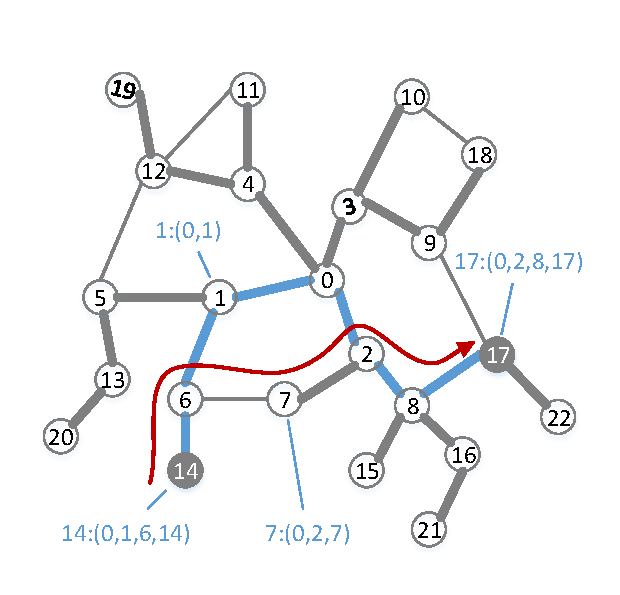
\epsfig{file=./figures/new_illustrate/ds_common.pdf,width=0.32\textwidth}\label{fig:DS:common}}
    %\subfigure[Bi-directional decentralized search]{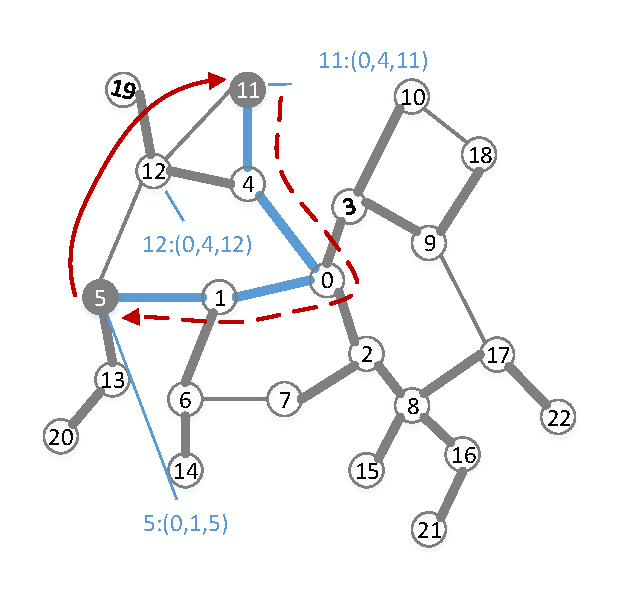
\epsfig{file=./figures/new_illustrate/ds_bidirectional.pdf,width=0.32\textwidth}\label{fig:DS:bidirectional}}
    %\subfigure[Tie breaking strategy]{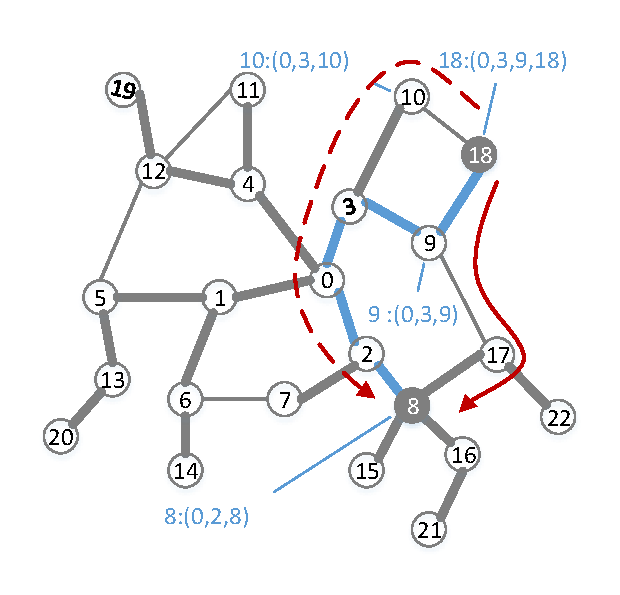
\epsfig{file=./figures/new_illustrate/ds_tie.pdf,width=0.32\textwidth}\label{fig:DS:tie}}
    %\caption{Examples of decentralized searches on indexed graphs. Bold lines denote the indexed edges. Curved lines denote paths being found, with arrows showing the directions. Dark vertices denote source and target vertices. Labels of vertices are shown in the $vertex:label$ format.}
%\end{figure*}

\begin{figure*}[ht]
		\vspace{-0.7cm}
    \centering
    \subfigure[Decentralized search 							 \label{fig:DS:common}]{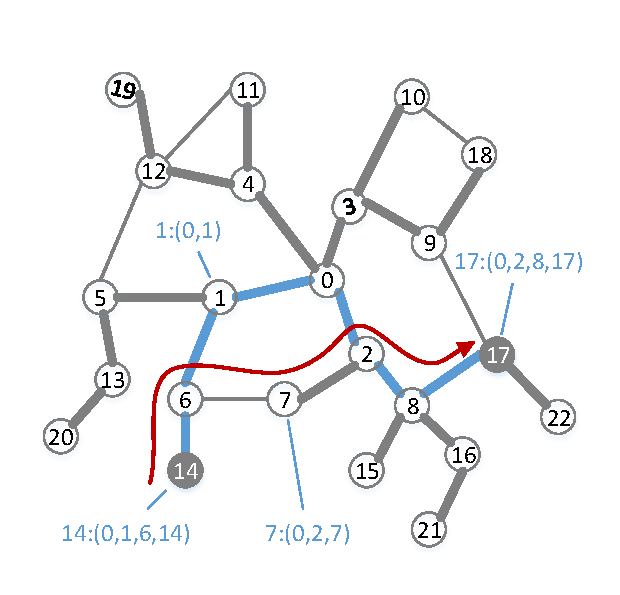
\includegraphics[width=0.32\textwidth]{figures/new_illustrate/ds_common.pdf}}
    \subfigure[Bi-directional decentralized search \label{fig:DS:bidirectional}]{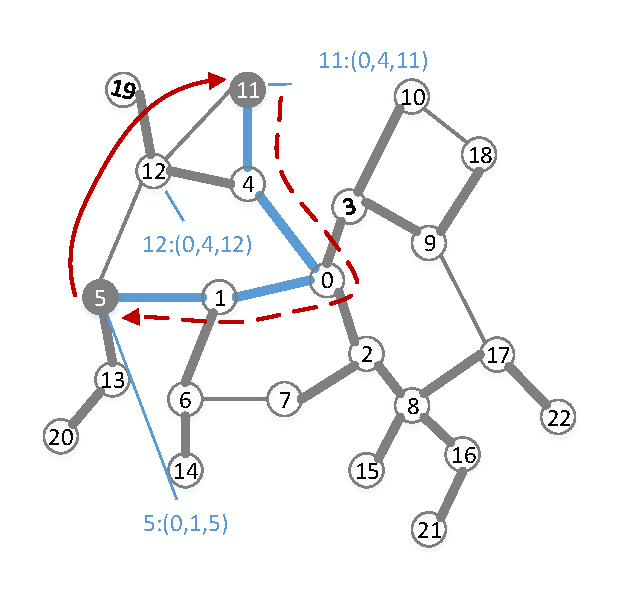
\includegraphics[width=0.32\textwidth]{figures/new_illustrate/ds_bidirectional.pdf}}
    \subfigure[Tie breaking strategy 							 \label{fig:DS:tie}]{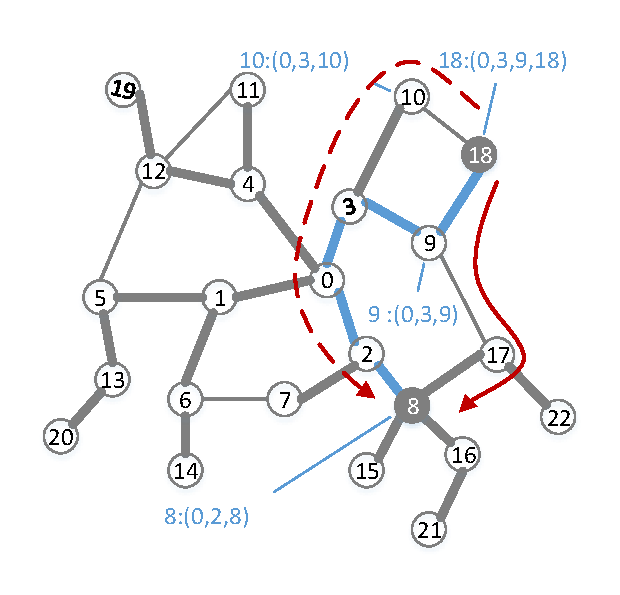
\includegraphics[width=0.32\textwidth]{figures/new_illustrate/ds_tie.pdf}}
    \caption{Examples of decentralized searches on indexed graphs. Bold lines denote the indexed edges. Curved lines denote paths being found, with arrows showing the directions. Dark vertices denote source and target vertices. Labels of vertices are shown in the $vertex:label$ format.}
\end{figure*}

We propose to solve the point-to-point shortest path approximation problem using decentralized search with landmark-based indexes. This section explains how to apply decentralized search on indexed graphs. Several aspects of the search, such as termination condition, bidirectional search and tie breaking strategy, are discussed.

\subsection{Preliminary}
In our problem, we consider a graph $G = (V,E)$. For a source node $s$ and a target node $t$, we are interested in finding a path $p(s,t)=(s,v_1,v_2,...,t)$ with a length of $|p(s,t)|$ close to the exact distance $d_G(s,t)$ between $s$ and $t$. We focus on unweighted, undirected graphs in this paper.

%Our method is motivated by the idea of using landmarks as the basis for indexes. Specifically, 
Given a graph $G$ and a set of $k$ landmarks $(l_1,l_2,...,l_k)$, an index contains a label $L(v)$ for each vertex that stores the shortest path to each landmark. The label can be constructed by building a shortest path tree $SPT$ using BFS from each landmark.

The least common ancestor of two vertices in a tree is the farthest ancestor from the root, which we denote as $LCA(s,t)$. The shortest distance satisfies the triangle inequality, i.e., for an arbitrary pair of vertices $s$ and $t$, the upper bound is $d_G(s,t) \leq min_{l}\{d_G(s,LCA_{l}(s,t)) + d_G(LCA_{l}(s,t),t)\}$.
We refer to this upper bound as the LCA distance and denoted by $d_{LCA}(s,t)$. We denote the path indicated by this distance as $p_{LCA}(s,t)$. 
%, can be used as an approximation of the distance from $s$ and $t$. 
%The LCA distance and related path for a specific landmark $l$ is denoted as $d_{LCA_l}(s,t)$ and $p_{LCA_l}(s,t)$ respectively.

\subsection{Index guided decentralized search}

To answer a shortest path query, decentralized search iteratively collects local distance information and visits the vertex with the least approximated distance to the target. More specifically, for a given pair of source $s$ and target vertex $t$ on an indexed graph, the search first sets the source vertex as the vertex to visit in the first step, and appends it to the approximated path $\tilde{p}(s,t)$. At each step, suppose that the search is visiting vertex $u$, it traverses all the neighbor vertices of $u$. For each neighbor vertex $v_i$, the metric $d_{LCA}(v_i,t)$ is calculated. Then the search sets the neighbor vertex with the smallest $d_{LCA}(v_i,t)$ as the vertex to visit in the next step, and appends $v_i$ to $\tilde{p}(s,t)$.

When the search reaches the target vertex, the search process naturally stops. However, this is not the ideal termination condition. We observe that, as shortest paths have optimal substructure, i.e., the path between any two vertices along a shortest path is also the shortest path of them, the search procedure can stop once it reaches an arbitrary vertex $u$, such that $u \in L(t)$ ($u$ is in the label of $t$. %meaning that a shortest path from $u$ to $t$ has been found). 
Evidently, decentralized search cannot find a shorter path than $p_L(u,t)$. The detailed algorithm of decentralized search is shown in Algorithm~\ref{alg:dec}.

\begin{algorithm}
    \caption{Decentralized search}
		\label{alg:dec}
    \begin{algorithmic}
        \Function{DecentralizedSearch}{$s$, $t$}
						\State $\tilde{p}(s,t) \gets \emptyset$
						\Comment {Initialize estimated path}
						\State $u \gets s$
						\State append $u$ to $\tilde{p}(s,t)$
						\While{$u \notin L(t)$}
								\State $d_{min} \gets \infty$
								\State $w \gets u$
								\For{each $v_i$ adjacent to $u$}
										\If{$d_{LCA}(v_i,t) < d_{min}$}
												\State $d_{min} \gets d_{LCA}(v_i,t)$
												\State $w \gets v_i$
										\EndIf
								\EndFor
								\State $u \gets w$
								\State append $u$ to $\tilde{p}(s,t)$
						\EndWhile
						\State $p_{remain} \gets p_L{u,t}$ excluding $u$
						\State append $p_{remain}$ to $\tilde{p}(s,t)$
						\State \Return $\tilde{p}(s,t)$
        \EndFunction
    \end{algorithmic}
\end{algorithm}

Observe that in this algorithm, by examining neighbor vertices, the search is able to explore a subset of the edges that are not indexed, to increase both accuracy and diversity of the path being found. For example, in Fig.~\ref{fig:DS:common}, observe that for the path from vertex $14$ to vertex $17$, decentralized search finds an edge $(6, 7)$ as vertex $7$ has a LCA distance of $3$, which is shorter than the LCA distance $5$ from vertex $1$ to $17$.

Regarding the termination condition, we have the following theorem:

\begin{theorem}
\label{theorem:max_step}
If the target vertex is reachable from the source, the decentralized search terminates in at most $2{\sigma}_{max}$ steps, where ${\sigma}_{max}$ is the diameter of the graph.
\end{theorem}
\begin{proof}[Proof Sketch]
For an arbitrary source vertex $s$ and a reachable target vertex $t$, the following bound holds:
\[
    d_{LCA}(s,t) = d_G(s,LCA(s,t)) + d_G(LCA(s,t),t) \leq 2{\sigma}_{max}
\]

Next, observe that at each step, decentralized search is visiting vertex $u$ and $u \neq t$. Assume the tightest upper bound shown above is achieved on the shortest path tree $SPT_l$ rooted at landmark $l$. Let $v$ be the neighbor vertex of $u$ on the path $p_{LCA_l}(u,t)$. Since $SPT_l$ has no cycles, $p_{LCA_l}(v,t) \in p_{LCA_l}(u,t)$. Therefore the following equation holds:
\[
		d_{LCA}(v,t) = |p_{LCA_l}(v,t)| = |p_{LCA_l}(u,t)| - 1 = d_{LCA}(u,t) - 1
\]
Since decentralized search always picks the neighbor with shortest LCA distance to the target, the LCA distance to the target at each step decreases at least by $1$. Therefore, the decentralized search terminates in at most $2{\sigma}_{max}$ steps.
\end{proof}

The time complexity of the decentralized search procedure depends on the maximum degree and the diameter of the graph. As decentralized search takes at most $2{\sigma}_{max}$ steps to finish and checks at most ${\delta}_{max}$ neighbor vertices at each step, where ${\delta}_{max}$ is the maximum vertex degree of the graph. For each neighbor, $k$ LCA computations are required, and the time complexity for each LCA computation is $O(h)$,
%$\footnote{$O(h)$, is for simple online algorithm, off-line algorithms can achieve time complexity of $O(1)$~\cite{bender2000lca}.}
where $h$ is the height of the indexed shortest path tree and $h \leq {\sigma}_{max}$. Therefore, the worst case time complexity of decentralized search is $O(k{{\sigma}_{max}}^2{\delta}_{max})$. 
%Based on our experiments on real-world graphs, decentralized search can finish in much fewer steps and check much fewer vertices at each step. Therefore, decentralized search can finish much faster in most cases.

The space complexity for decentralized search contains two parts, space complexity for offline indexing, and space complexity for online query. The space required for offline indexing is $O(k{\sigma}_{max}n)$, where $n$ is the number of vertices. 
%For each query, $O(k{\sigma}_{max})$ space is required to store the labels of target vertex and the vertex that is being examined. Therefore, $O(2{\sigma}_{max})$ space is required to store the approximated path. Combining them together, 
The online search space complexity of decentralized search is $O(k{\sigma}_{max})$.

\subsection{Bi-directional search}

In this section, we show how to apply the idea of bidirectional search to decentralized search. In bidirectional decentralized search, the backward search starts at the target vertex and is driven by the goal to reach the source vertex. The forward search and backward search may explore different search spaces due to this difference. By exploring a different search space, the backward search may find a shorter approximated path. This, however, is quite different from the application of bidirectional search in BFS or A* search where the main focus is to reduce search space. It is not guaranteed that the forward search and the backward search will eventually meet at any intermediate vertex. 

An example of directional decentralized search is shown in Fig.~\ref{fig:DS:bidirectional}. Let $11$ be the source and $5$ be the target. The backward search can find a shorter path $p_{bwd} = (5, 12, 11)$ than the path $p_{fwd} = (11, 4, 0, 1, 5)$ by the forward search. The backward search finds a shorter path by exploring edge $(5, 12)$. However, this edge is invisible to the forward search because when the search traverses vertex $4$, it prioritizes $0$ than $12$ due to the former one has a lower LDA distance to the target vertex $5$.

%As shown in our previous example, $p_{fwd} \cap p_{bwd} = (11, 5)$. Actually, in decentralized search, the forward search and backward search are mostly two independent searches, where the only interaction of them is when the search results are combined, where the shorter paths are returned. 

\subsection{Tie breaking strategy}

Ties happen frequently in decentralized search, especially when the number of landmarks is small. In the decentralized search, a tie means multiple neighbor vertices have same LCA distance to the target in a step. 
%The reason that a tie happens is that there is not sufficient information in indexes that can separate neighbor vertices for a query. 
For example, in Fig.~\ref{fig:DS:tie}, consider a search from $18$ to $8$. When traversing neighbors of vertex $18$, both vertex $10$ and $9$ have the same LCA distances to target vertex $8$, but their actual distances to vertex $8$ are different, due to that the shortcut edge $(9, 17)$ is currently invisible to the decentralized search.

The search space of the decentralized search can be increased by expanding the search onto each tied vertex. This increases both the performance, i.e., chances to find a shorter path and the number of paths being found, and the cost of the search. By controlling the search space this way, decentralized search is able to achieve different levels of accuracy.

%Two extreme ways to deal with ties are either only visiting one vertex, or visiting all vertices in the next step. The former one incurs the least search cost, and has the least possibility to find a shorter path. We refer to it as single branch decentralized search. The latter one requires most effort and can lead to the shortest path the decentralized search could possibly find. We refer to it as full branch decentralized search.

%\subsection{Extension on directed graphs}
%To treat directed graphs, for each landmark, the label of a vertex $u$ need to store both the path from the landmark to the vertex, denoted as $p_{l \rightarrow u}$, and the path from the vertex to the landmark, denoted as $p_{u \rightarrow l}$. When the search is visiting vertex $u$, only out-edges of $u$ need to be traversed. To calculate LCA distance from $u$ to the target vertex $t$, $p_{l \rightarrow u}$ is used for $u$ and $p_{t \rightarrow l}$ is used.

\section{Index Construction}
\label{preprocessing}

This section describes our index construction algorithm. Previous works have studied various landmark selection strategies which have a significant impact on the accuracy of online query. In our study, we observe that even with the same landmark set, choosing which shortest path from vertex to landmark to be indexed also plays an important role for the accuracy of online search. 

\begin{figure*}[ht]
    \centering
    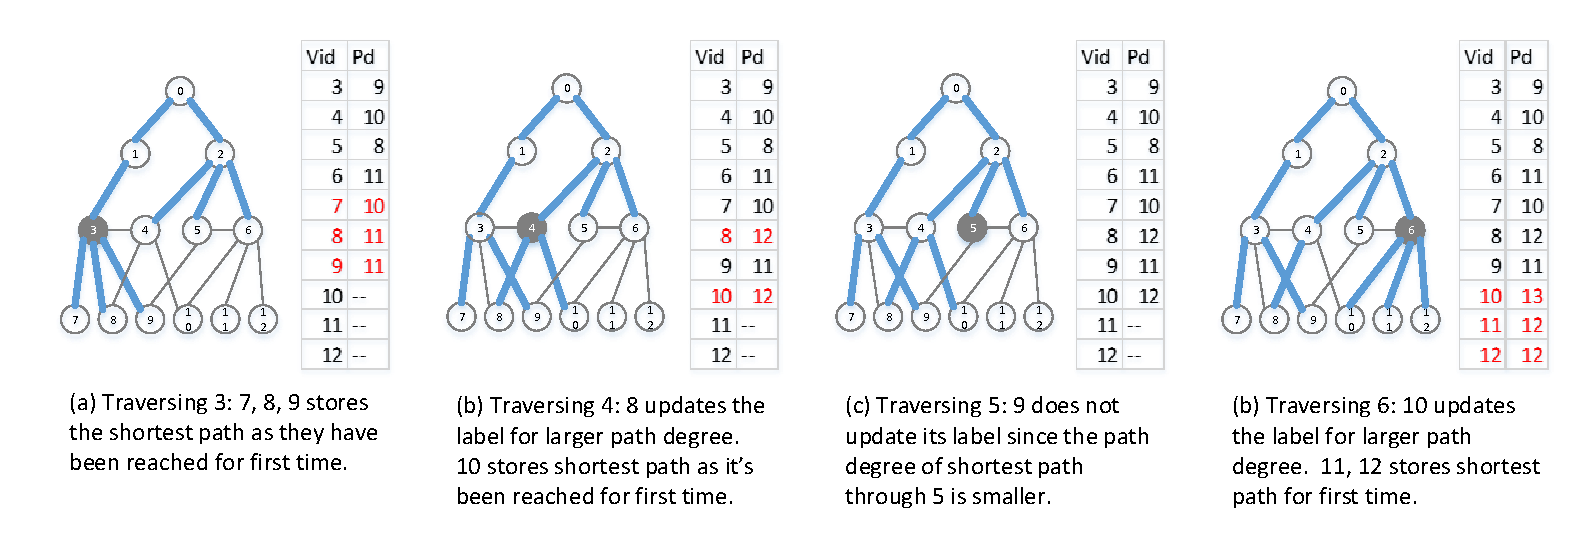
\includegraphics[width=\linewidth]{./figures/new_illustrate/bfs_illustrate.pdf}
    \caption{Greedy algorithm that index shortest path with highest path degree during breadth first search}
    \label{fig:bfs_illustrate}
\end{figure*}

\subsection{Greedy index construction algorithm}
\begin{algorithm}
    \caption{Algorithm greedy index construction vertex program running on $u$}
		\label{alg:ind}
    \begin{algorithmic}
				\Function{Index construction}{$root$}
					\State $PD \gets \emptyset$
					\State $L \gets \emptyset$
					\State $Q \gets \emptyset$
					\State $L[root.id] = root.id$
					\State $PD[root.id] = root.degree$
					\State $Q.push(root)$
					\While{$Q \neq \emptyset$}
						\State $u = Q.pop()$
						\For{$each v adjecent to u$}
							\If{$v.id \not \in L$}
								\State $L[v.id] = L[u.id] \cup v.id$
								\State $PD[v.id] = PD[u.id] + u.degree$
								\State $Q.push(v)$
							\ElsIf{$L(v).size() < L(u).size() + 1$}
								\State $continue$
							\ElsIf{PD[v.id] < PD[u.id] + u.degree}
								\State $L[v.id] = L[u.id] \cup v.id$
								\State $PD[v.id] = PD[u.id] + u.degree$
							\EndIf
						\EndFor
					\EndWhile
					\State \Return $L$
        \EndFunction
    \end{algorithmic}
\end{algorithm}

On the core of decentralized search is to iteratively find vertices that share the least common ancestor with target vertex at a higher level of the indexed shortest path tree. From the point of view of a vertex, a good shortest path from each landmark to be indexed should be the one that intersects with most of other shortest paths. As the more intersects with other shortest paths, the higher the chance there exist a LCA at a higher level for average cases. With this intuition, we design our heuristic greedy index construction algorithm to index the shortest path with highest "centrality", i.e. intersects with most other shortest paths. To represent the "centrality" of a shortest path, we use the sum of vertex centrality along the path. Betweenness centrality fits our needs very well as it directly represent number of shortest paths each vertex on, but the computation complexity to even estimate the value for every vertex in a graph is still high ~\cite{Riondato:2014:FAB:2556195.2556224}. So we use degree as an alternative and refer the sum of degree of vertices along a path as path degree, denoted by $Pd$.

Our greedy index construction algorithm, which greedily index shortest paths with highest path degree, can be easily modified from the regular index construction procedure. Note that path degree of shortest path follows optimal substructure, i.e. if $(u, .., w, ..., v)$ has the highest path degree among all the shortest path from $u$ to $v$, then the path degree of $(u, ..., w)$ is also the highest among all the shortest path from $u$ to $w$. Normally, the index is constructed with a BFS and a label is assigned to each node the first time the search reach it. To modify it, we first need to add a variable to cache the path degree $Pd$ of the shortest path stored in the label of each vertex. Then during BFS traversal, suppose the search is visiting vertex $u$ and reach its neighbor $v$. If $L(v)$ is not empty, and $v$ is on a higher level of BFS tree than $u$, then a label update is performed. If $Pd(u) + v.degree > Pd(v)$, then the label and related path degree of $v$ are updated. Fig. \ref{fig:bfs_illustrate} shows an example of how to greedily select shortest path with the highest path degree during breadth first search. When traversing vertex $4$, even though vertex $8$ has already been indexed with a shortest path $(0, 1, 3, 8)$ into its label, due to that $(0, 2, 4, 8)$ has a higher path degree, the label of vertex $8$ is updated. The same thing happens to vertex $10$ while traversing vertex $6$.

The detailed algorithm of greedy index construction is depicted in \ref{alg:dec}.
\section{Distributed Implementations}
\label{implementation}

To handle extremely large graphs and large amount of queries, we implement our algorithm in distributed settings. Since decentralized search has low online search space complexity and does not have data dependency upon each other, it is well suitable to run in a parallel way. In this section, we discuss how to implement decentralized search on a distributed general graph processing platform, Powergraph\cite{180251}.

\begin{figure*}[ht]
    \centering
    \includegraphics[width=\linewidth]{./figures/new_illustrate/System.pdf}
    \caption{A system overview}
    \label{fig:system}
\end{figure*}

\subsection{Decentralized search vertex-program}

An overview of our shortest path query processing system is shown in \ref{fig:system}. The system first partition the graph with Powergraph onto multiple machines. Then several BFSs are performed to construct the index. After the index is built, multiple shortest path queries can run in parallel with decentralized search. Large volumes of queries can submit repeatedly, for which responses will be generated.

Decentralized search can be easily implemented as vertex-program in appliance to Powergraph's Gather-Apply-Scatter model. Each search instance contains approximated path and label of target vertex, as index is stored distributively and label of target vertex may not be accessible on each machine locally. In Gather phase, the search aim to find the neighbor with shortest LCA distance to the target. For each query, LCA distance $d_LCA$ calculated from labels $L$ of each neighbor and target vertex is collected and accumulated by finding the neighbor with the smallest LCA distance, A next hop candidate is returned after this phase. In apply phase, the program appends the candidate to the approximated path $p_{appr.}$ and and check whether the terminate criteria is met for each query. If so, the result path will be recorded and the query will be terminated. Otherwise, program will proceed to Scatter phase to start new vertex-programs on the candidate vertex and pass on the query instance to them. Algorithm \ref{alg:vc_dec} shows the detailed algorithm.

\begin{algorithm}
    \caption{Algorithm decentralized search vertex program running on $u$}
		\label{alg:vc_dec}
    \begin{algorithmic}
        \Function{gather}{$L(v)$, $L(t)$}
        %\Comment {Collect LCA distances from Nbrs}
        \State \Return $d_LCA(v, t)$, $v.id$
        \EndFunction

        \Function{sum}{$d_LCA(v_1,t)$, $vid1$, $d_LCA(v_2,t)$, $vid2$}
        %\Comment {Find Nbr with smallest LCA distance to target}
        \State \Return $min(d_LCA(v_1,t), d_LCA(v_2,t)$, related $vid$
        \EndFunction

        \Function{apply}{$p_{appr.}(s,t)$, $d_LCA(v,t)$}
        %\Comment {Update approximate path and check termination}
        \State $p_{appr.}(s,t) += vid$
        \If {terminate criteria is met}
            \State store $p_{appr.}(s,t)$
            \State $term$ = true
        \Else
            \State $term$ = false
        \EndIf
        \EndFunction

        \Function{scatter}{$p_{appr.}(s,t)$, $term$}
        %\Comment {activate candidates}
        \If {$\neg term$}
            \State Activate(v, $p_{appr.}(s,t)$)
        \EndIf
        \EndFunction
    \end{algorithmic}
\end{algorithm}

There are two thing to notice for the decentralized search vertex program. First, the search only update the approximated path $p_{appr.}$. There is no data dependency among multiple searches except when in the last results are stored to the same container for each machine. Second, the communication for decentralized search can happen during gather and scatter phase. In gather phase, the label of target vertex need to be passed to multiple machines, and the size is $O(k{\sigma}_{max})$. And each gather function return a $d_LCA$ along with its id that has $O(1)$ size. So for each query, only $(O(k{\sigma}_{max}) + O(1)) * M$ size of data is transferred where $M$ is the number of machines. In scatter phase, communication happens when a vertex is chosen as next hop and need to be activated, the whole search instance, including approximated path and label of target vertex need be transmitted to the new vertex program. For each query, $O(k{\sigma}_{max}) + O({\sigma}_{max})$ size of data may be transferred.

The low memory and communication cost, along side with light data dependency makes multiple decentralized search instance very suitable to run in parallel. To modify the vertex program for parallel processing, each vertex program maintain a list of search instance. During gather phase, label of target vertex for each query is transmitted to other machines, and $d_LCA$ is calculated for each query. Each query is updated during apply phase. In scatter phase, each query is examined for whether activating a certain vertex or not.

\subsection{Distributed tie breaking strategy}
If a tie happens, according to tie strategy, multiple neighbors may be returned as candidates at gather phase. Then at apply phase, the search instance will be fork itself into multiple search instance, each for a single candidate. The problem here is, not like centralized version, during the future computation, even a search instance find a shorter path than others, it cannot terminate other searches as such synchronization is quite costly in distributed settings. With this limitation, the search space are quite difficult to control and the search may end up with excessive number of child search instances. So in our implementation, at each step, only one candidate will be chosen as a "`main"' candidate. For candidates that are not "`main"' candidates, an extra terminate criteria will be applied. At the next step, if the search cannot find a shorter path than expected, i.e. $|p_{appr.}| + d_LCA$, then the search will stop, and no result will be recorded. This can control the search space effectively without compromise accuracy too much.

\subsection{Prune LCA computation}
It is possible to prune number of LCA computation required at each step for decentralized search. Suppose the search is visiting vertex $u$, which means the $d_LCA{u, t}$ has already been calculated in previous step. When traverse $u$'s neighbors, if a neighbor $v$ is a child on the indexed shortest path tree $T_i$, then the LCA computation for $v$ and $t$ on that tree $T_i$ does not need to be performed as it is certain that $d_LCA(i){v, t} > d_LCA(i){u, t}$. In practice, such way to pruning can reduce half of the total number of LCA computations of a single search on average.

\section{System Evaluation}
\label{evaluation}

\subsection{Evaluation Overview}
 
\subsection{Datasets}
 
\subsection{Methodology}
 
 
\subsection{Evaluation Results}
 
\section{Conclusion}
\label{conclusion}

In this paper, we describe a novel method to combine online and offline processing to allow approximate shortest path searches for extremely large graphs with high distance accuracy, path diversity and low overhead. We demonstrate that different accuracy and overhead levels can be achieved by controlling the search space of decentralized searches. We also propose a more effective heuristic approach for constructing indexes of the network that can improve the accuracy of the decentralized search without increasing preprocessing and online searching overhead. We implement our algorithm for cloud computing graph processing platforms, and demonstrate that our system can handle extremely large graphs and processing millions of queries in parallel.


% The following two commands are all you need in the
% initial runs of your .tex file to
% produce the bibliography for the citations in your paper.
\bibliographystyle{abbrv}
%{\footnotesize
%\bibliography{reference}}
\bibliography{reference}
% You must have a proper ".bib" file
%  and remember to run:
% latex bibtex latex latex
% to resolve all references
%
% ACM needs 'a single self-contained file'!
%
%APPENDICES are optional
%\balancecolumns

% That's all folks!
\end{document}
